\documentclass[11pt]{article}

% --- packages ---
\usepackage[margin=1in]{geometry}
\usepackage{graphicx}
\usepackage{booktabs}
\usepackage{array}
\usepackage{amsmath,amssymb}
\usepackage{textcomp}
\usepackage{authblk}
\usepackage[hidelinks]{hyperref}
\usepackage{caption}
\usepackage{subcaption}
\captionsetup{font=small,labelfont=bf}
\renewcommand{\thesubfigure}{\Alph{subfigure}}  % panel labels A, B

% --- convenience macros for recurring symbols (engine-agnostic) ---
\newcommand{\uOR}{\textmu-opioid receptor}
\newcommand{\uor}{\textmu-opioid}
\newcommand{\Ang}{\AA}
\newcommand{\Angsq}{\AA\textsuperscript{2}}
\newcommand{\bt}{$\beta$}
\newcommand{\al}{$\alpha$}
\newcommand{\gm}{$\gamma$}
\newcommand{\pistack}{$\pi$}
\newcommand{\x}{$\times$}
\newcommand{\lteq}{$\le$}
\newcommand{\ra}{$\rightarrow$}
\newcommand{\approxx}{$\approx$}
\newcommand{\ca}{$\sim$}

\title{\vspace{-2em}\bfseries Structural basis of ZH853 recognition by the \uor{} receptor:
a distinctive extracellular-loop contact defines a selectivity handle and guides analog design}

\author[1]{M. J. O'Meara \emph{et al.}}
\affil[1]{Department of Computational Medicine and Bioinformatics, University of Michigan}
\date{Working draft, 22 July 2026}

\begin{document}
\maketitle

\noindent\small\emph{Status:} Results for Objectives 1--3 are complete; the molecular-dynamics and
free-energy validation (Methods \S2.5) is prepared but not yet run --- claims dependent on it are
flagged \textbf{[prospective]}.\normalsize

\begin{abstract}
\noindent The cyclic endomorphin-1 analog ZH853 is a potent \uOR{} (MOR) agonist with an attractive
preclinical profile, but the structural basis of its binding --- and how it differs from other opioid
agonists --- has not been characterized. Using a 3.5\,\Ang{} cryo-EM structure of the
MOR--ZH853--Gi--scFv16 complex, we computed heavy-atom interaction fingerprints for ZH853 and
benchmarked them against thirteen deposited MOR complexes spanning peptide agonists (DAMGO,
endomorphin-1, \bt-endorphin), morphinan and fentanyl-class small molecules, biased agonists, and an
antagonist. ZH853 engages the canonical opioid anchor (a salt bridge to Asp3.32 satisfied by its Tyr1
\al-amine, plus the Tyr7.43 ``3--7 lock'') shared by all agonists, but additionally forms a
\textbf{salt bridge to Glu231 in extracellular loop 2 (ECL2) that no other agonist in the set makes},
together with an aromatic/cation-\pistack{} contact to His7.36 shared only with its endomorphin-1
parent. This extended ECL2/ECL3 engagement is the structural signature of the cyclic scaffold. We
nominate \textbf{E231Q/E231A} as mutations predicted to disrupt ZH853 selectively while sparing
related full agonists, and identify the molecule's beyond-rule-of-5 liabilities (TPSA 235--280\,\Angsq,
8--10 H-bond donors), proposing two orthogonal optimization series --- backbone N-methylation for
passive permeability and semaglutide-style C-terminal lipidation for half-life --- targeted to
solvent-exposed positions established from the bound pose. A membrane molecular-dynamics and
free-energy protocol to test these hypotheses is established and released. This is, to our knowledge,
the first structural analysis of a cyclic-peptide MOR complex.
\end{abstract}

\section{Introduction}

Opioid analgesics acting at the \uOR{} (MOR, gene \emph{OPRM1}) remain the mainstay of severe pain
management, but their utility is limited by respiratory depression, tolerance, and dependence. A
central goal of contemporary opioid pharmacology is to retain analgesic efficacy while separating it
from these liabilities --- through signaling bias, partial agonism, or novel chemotypes. Endomorphins,
the endogenous MOR-selective tetrapeptides (Tyr-Pro-Trp-Phe-NH$_2$), are attractive scaffolds because
of their high selectivity, but their linear form is metabolically labile and poorly bioavailable. The
Zadina laboratory addressed this by engineering cyclic, D-amino-acid endomorphin analogs;
\textbf{ZH853} (Tyr-cyclo[D-Lys-Trp-Phe-Glu]-Gly-NH$_2$) is a lead from this series with potent
antinociception and a reduced side-effect profile in rodents [1].

Despite this promise, no structure of ZH853 --- or of any cyclic-peptide MOR complex --- has been
reported, leaving open three questions this work addresses computationally from a 3.5\,\Ang{} cryo-EM
structure of the MOR--ZH853--Gi--scFv16 complex (Figure~\ref{fig:complex}): (1) \emph{what, if anything,
is structurally
distinctive about how ZH853 engages MOR} relative to other agonists; (2) \emph{which receptor
mutations would abrogate ZH853 while sparing related full agonists}, providing a pharmacological
fingerprint and a route to mechanistic tests; and (3) \emph{how ZH853's drug-like properties could be
improved}, drawing on modern peptide-drug strategies. We further establish and release a membrane
molecular-dynamics (MD) and free-energy protocol to validate these structure-derived hypotheses.

\begin{figure}[t]
  \centering
  \begin{subfigure}[b]{0.365\textwidth}
    \centering
    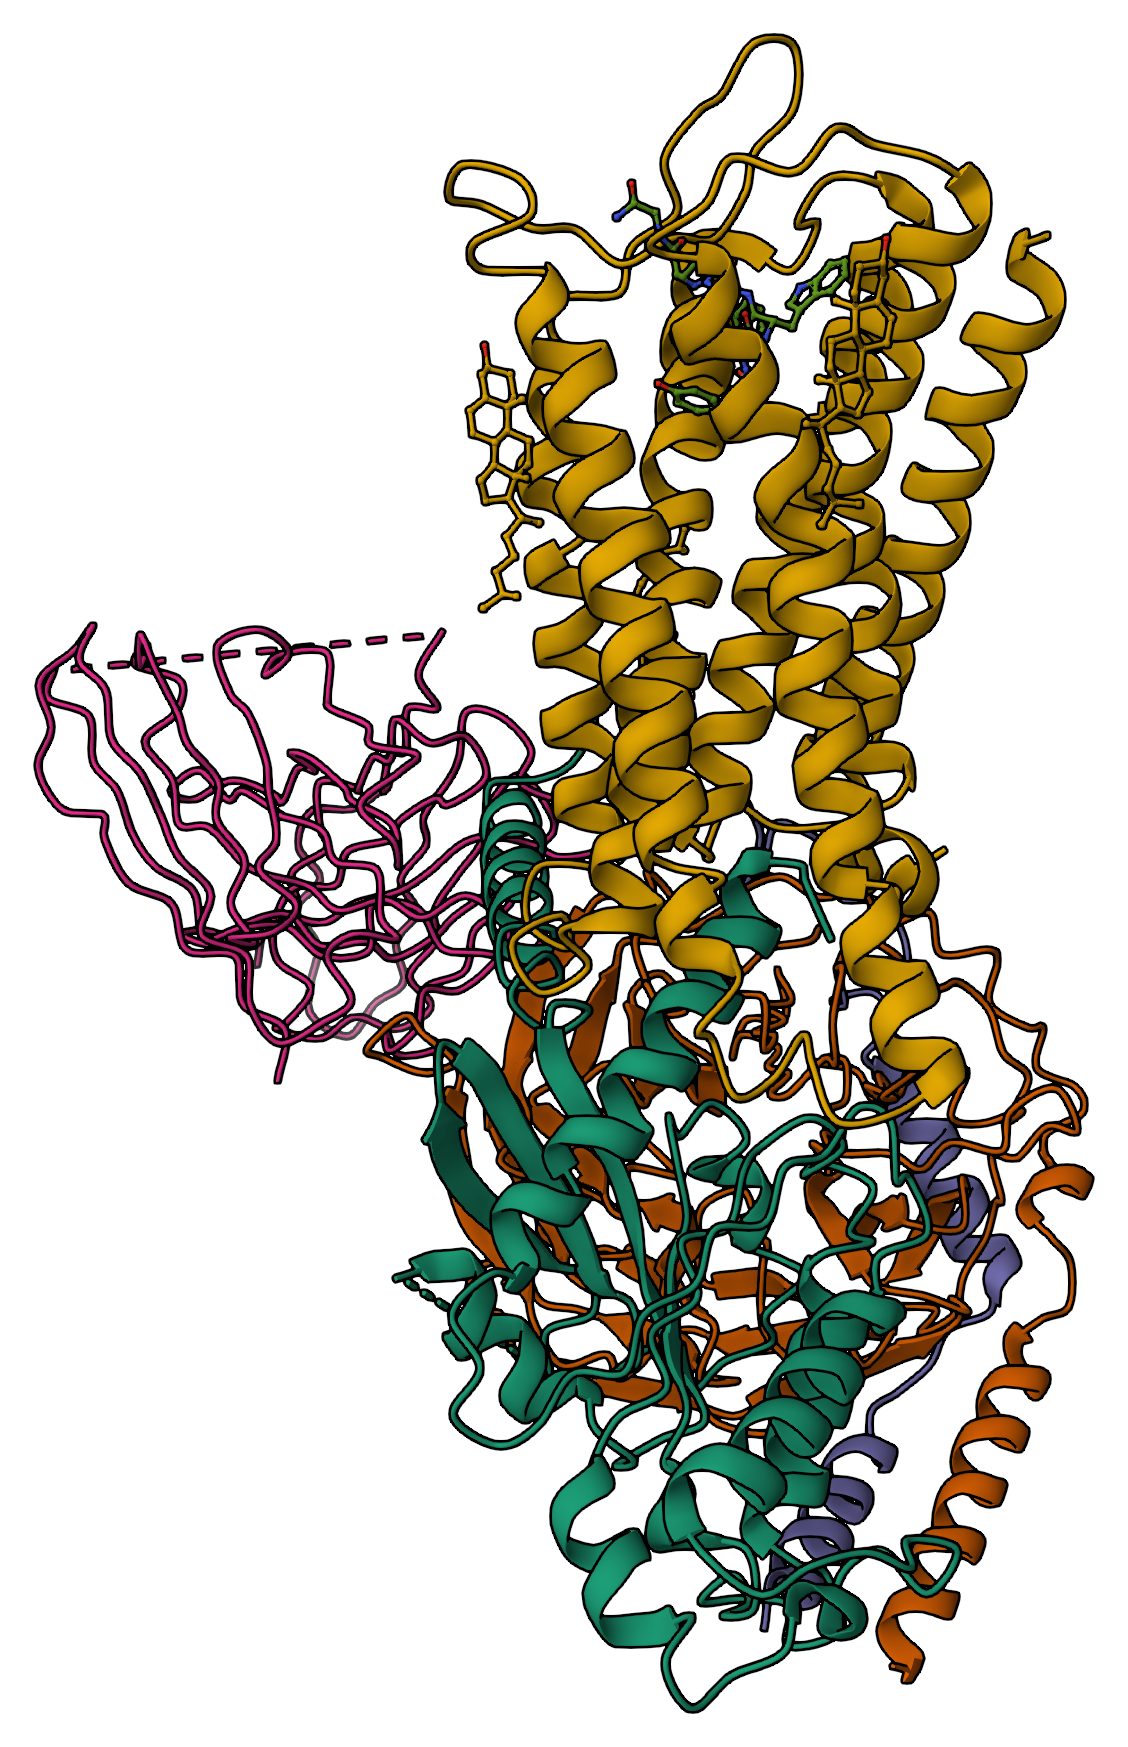
\includegraphics[width=\linewidth]{figures/fig6_molstar_overview.png}
    \caption{}\label{fig:complex-a}
  \end{subfigure}\hfill
  \begin{subfigure}[b]{0.60\textwidth}
    \centering
    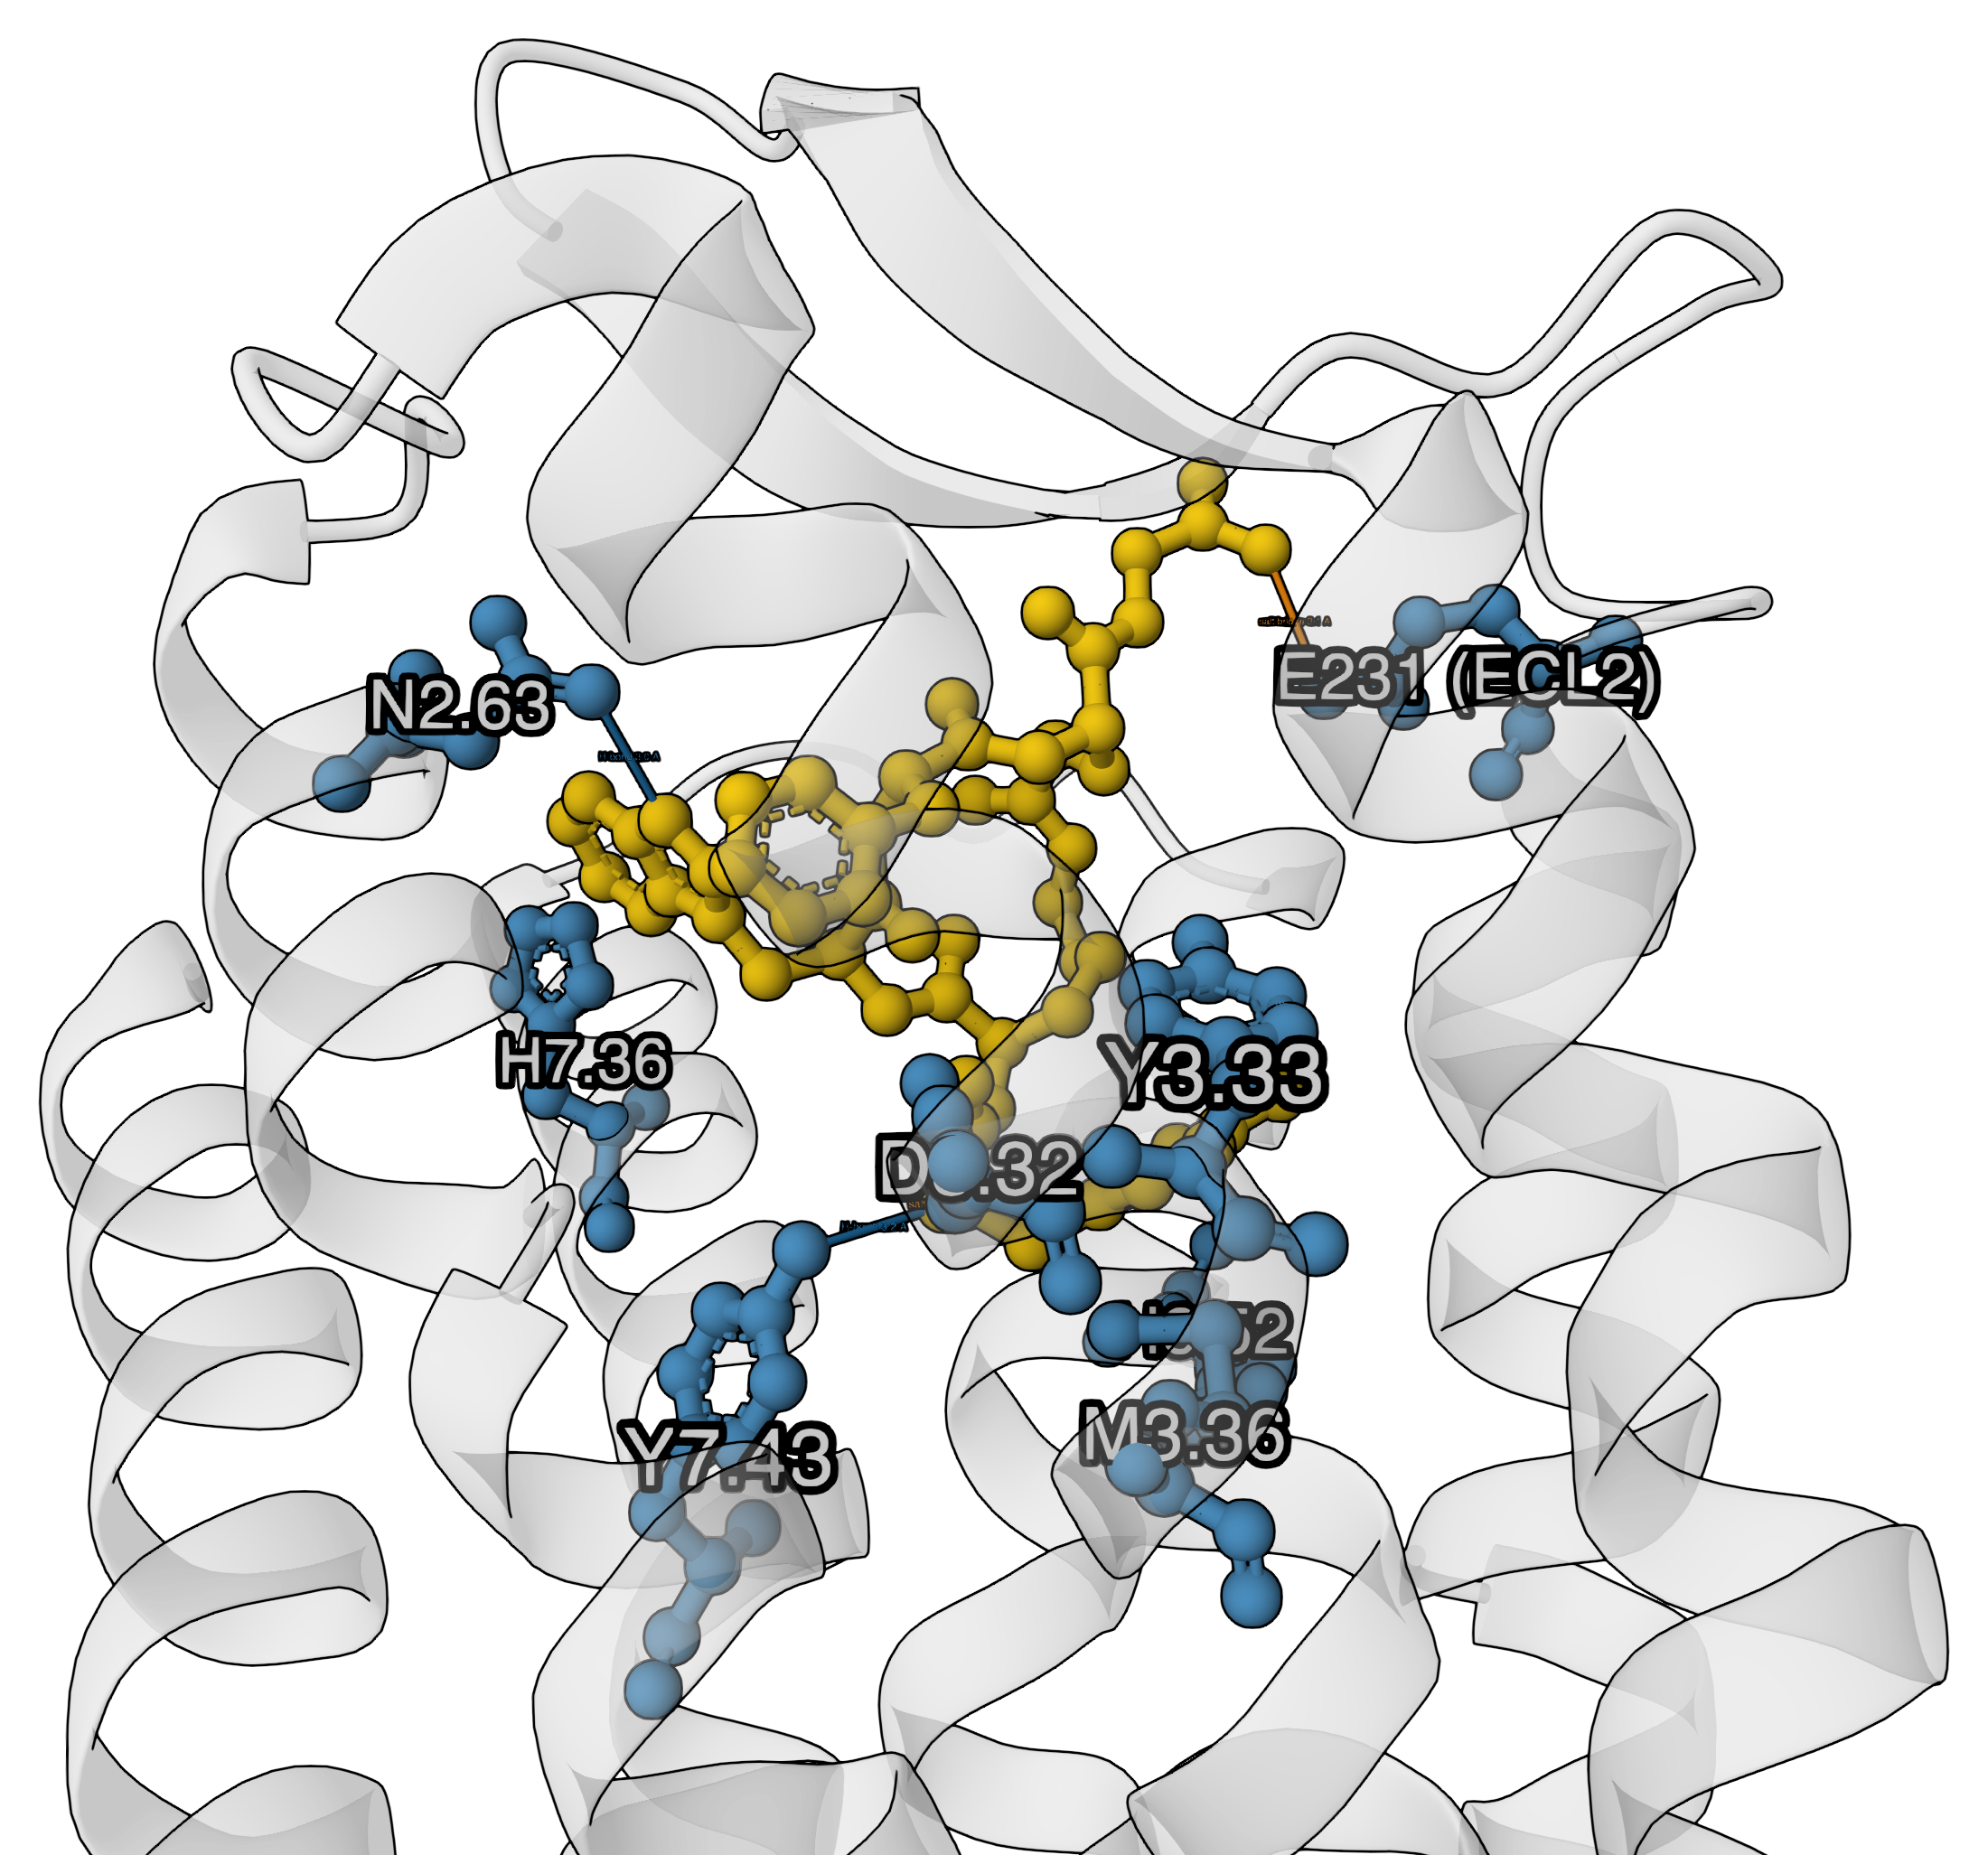
\includegraphics[width=\linewidth]{figures/fig7_molstar_pocket.png}
    \caption{}\label{fig:complex-b}
  \end{subfigure}
  \caption{The experimentally characterized MOR--ZH853--Gi--scFv16 cryo-EM complex (Mol* renders).
  \textbf{(A)} The whole complex in the canonical GPCR orientation --- extracellular face up,
  intracellular G-protein interface down: \uOR{} receptor 7TM bundle (gold, top) with ZH853
  (green sticks) in the extracellular orthosteric pocket, coupling to G$\alpha$i (orange),
  G$\beta$ (teal) and G$\gamma$ (purple), with the scFv16 fragment (magenta).
  \textbf{(B)} The orthosteric pocket: ZH853 (yellow ball-and-stick) with key receptor residues (blue)
  as sticks, labeled by Ballesteros-Weinstein number; salt bridges (orange) to Asp3.32 and ECL2
  Glu231 and H-bonds (blue) to Tyr7.43 and Asn2.63 are drawn as distance lines, the receptor cartoon
  faded for context.}
  \label{fig:complex}
\end{figure}

\section{Related work}

\textbf{MOR structural pharmacology.} The inactive MOR structure (\bt-FNA, 4DKL [2]) and the active
BU72 complex (5C1M [3]) established the orthosteric pocket and the activation-associated rearrangements
of the W6.48 toggle and TM6. Cryo-EM of MOR--Gi complexes then resolved a series of agonists --- the
peptide DAMGO (6DDE [4]; human 8EFQ) and endomorphin-1/\bt-endorphin (8F7R/8F7Q [7]), and the small
molecules fentanyl, morphine, oliceridine, SR-17018, PZM21 (8EF5/8EF6/8EFB/8EFL/8EFO [5]) and
mitragynine pseudoindoxyl/lofentanil (7T2G/7T2H [6]). All share the D3.32 anchor and a conserved
hydrophobic subpocket; biased agonists differ mainly in TM6/ECL2 engagement. Notably, \emph{every}
deposited peptide-agonist MOR structure carries a \emph{linear} peptide --- ZH853 would be the first
cyclic-peptide complex.

\textbf{Cyclic peptides as drugs.} Macrocyclic peptides occupy ``beyond-rule-of-5'' (bRo5) chemical
space [9]; their oral/passive permeability is governed less by static polarity than by conformational
shielding of backbone donors (``molecular chameleons'' [10]), which N-methylation and cyclization
promote (as in cyclosporine). Half-life, by contrast, is engineered through albumin-binding
\textbf{lipidation} --- the strategy that gives semaglutide a \ca1-week half-life via a
\gm Glu-2\x AEEA-C18-diacid conjugate [11]. These two axes --- permeability and duration --- are
distinct and are treated separately here.

\section{Methods}

\textbf{3.1 Structure and numbering.} We used the deposited real-space-refined MOR--Gi--scFv16--ZH853
model (3.5\,\Ang; CC$_{\text{mask}}$ 0.80; 0.0\% Ramachandran outliers). Chains: G\al i (A), G\bt 1
(B), G\gm 2 (C), scFv16 (D), MOR/\emph{OPRM1} residues 69--349 with 84 modeled cholesterols (R), and
ZH853 as HETATM ligand L01 (E). The construct uses \textbf{human OPRM1 (UniProt P35372) numbering},
verified against all canonical orthosteric positions; mouse-numbered comparators were offset by $+2$
to this frame. The ligand's 59 heavy atoms and formula (C$_{42}$H$_{51}$N$_9$O$_8$, 810\,Da) match the
reference SMILES, confirming the monomeric macrocycle. The overall complex and the orthosteric pocket
are shown in Figure~\ref{fig:complex}A,B.

\textbf{3.2 Comparator set.} Thirteen structures were retrieved from the RCSB PDB: peptide agonists
6DDE/8EFQ (DAMGO), 8F7R (endomorphin-1), 8F7Q (\bt-endorphin), 9WST/9WSV (DAMGO with Gz/\bt-arrestin);
small molecules 5C1M (BU72), 8EF5 (fentanyl), 8EFB (oliceridine), 8EFL (SR-17018), 8EFO (PZM21), 7T2G
(mitragynine pseudoindoxyl); and antagonist 4DKL (\bt-FNA). For each, the receptor chain and bound
agonist were isolated programmatically and mapped to human OPRM1 numbering.

\textbf{3.3 Interaction fingerprints.} Because the 3.5\,\Ang{} model lacks hydrogens, we used a
resolution-matched \textbf{heavy-atom geometric fingerprint} (rather than angle-based H-bond criteria),
classifying each receptor--ligand residue contact as ionic (opposite-charge groups \lteq4.0\,\Ang),
H-bond (polar N/O \lteq3.5\,\Ang), hydrophobic (C--C \lteq4.0\,\Ang), \pistack-stacking (aromatic
centroids \lteq5.5\,\Ang), or cation-\pistack{} (\lteq6.0\,\Ang). Aromatic rings of non-standard ligands
were detected by planar-ring geometry, a template-free method that generalizes across chemotypes. The
same method was applied uniformly to all fourteen complexes.

\textbf{3.4 Mutation panel and cheminformatics.} Candidate selectivity mutations were scored by ZH853
interaction strength \x{} rarity across the twelve agonists \x{} a bonus for sparing the two closest
full agonists (endomorphin-1, DAMGO). Physicochemical descriptors (2D, plus 3D radius of gyration,
polar SASA fraction, and intramolecular H-bond count from macrocycle-aware conformers) were computed
with RDKit; modification variants (N-methylation, lipid conjugation, halogenation) were enumerated
programmatically and their properties predicted. Buried vs solvent-exposed ligand atoms were
determined from the bound pose (\lteq4.5\,\Ang{} to receptor).

\textbf{3.5 MD/free-energy protocol [prospective].} A membrane MD system was prepared: receptor
sidechains rebuilt (PDBFixer), protonation assigned by PROPKA at pH 7.4, and ZH853 protonated to $+1$
and prepared for GAFF2/RESP parameterization. PROPKA places \textbf{D2.50 (Asp116) at pKa 7.61}, so
parallel protonated/charged systems are built. The production protocol (POPC:cholesterol 9:1,
ff19SB/Lipid21/OPC, CHARMM-GUI-style six-stage equilibration, LangevinMiddle 310\,K with a
semi-isotropic membrane barostat, hydrogen-mass repartitioning at 4\,fs, $\ge$3 replicas) and
free-energy calculations (relative FEP across the ZH850/831/809 analogs; ABFE and funnel metadynamics
as exploratory) are released as a SLURM bundle. Given documented convergence difficulties for flexible
macrocycles, free-energy results are framed as rank-ordering.

\emph{All analyses are scripted and version-controlled (Data \& code availability).}

\section{Results}

\subsection{ZH853 satisfies the conserved opioid anchor}

ZH853 contacts 25 receptor residues. Its Tyr1 \al-amine forms the \textbf{canonical Asp3.32 (Asp149)
salt bridge} (3.16\,\Ang) and hydrogen-bonds Tyr7.43 (Tyr328, 3.17\,\Ang) --- the ``3--7 lock'' ---
while the Tyr1 ring and the macrocyclic Trp/Phe pack into the conserved hydrophobic subpocket (Met3.36,
Val3.28/Ile3.29, Ile6.51, Val6.55, Val5.42; Figure~\ref{fig:posemap}). Every one of these contacts is
shared by all twelve comparator agonists (Figure~\ref{fig:heatmap}), confirming that ZH853 presents the
same ``message''
pharmacophore as morphine, fentanyl, DAMGO, and endomorphin-1. Consistent with this, PROPKA assigns
Asp149 a depressed pKa (6.0), i.e.\ charged and salt-bridge-competent.

\subsection{A distinctive ECL2 salt bridge distinguishes ZH853 (Objective 1)}

Against this conserved background, three contacts set ZH853 apart (Figure~\ref{fig:heatmap};
Table~\ref{tab:distinctive}):
\begin{itemize}
  \item \textbf{Glu231 (ECL2): an ionic + H-bond contact made by ZH853 alone (0/12 agonists).} A ZH853
  basic group reaches ECL2 to form a salt bridge (3.12\,\Ang) that no linear peptide or small molecule
  in the set reproduces. PROPKA confirms Glu231 is charged (pKa 4.9). This is the single strongest
  structural discriminator.
  \item \textbf{His7.36 (His321): aromatic/cation-\pistack, shared only with endomorphin-1 and
  mitragynine (2/12).} An ECL3-proximal contact retained from the endomorphin-1 lineage.
  \item Weaker ZH853-unique contacts at Leu221/Phe223 (ECL2) and Leu234 (TM5), gained by the
  extended/cyclic scaffold.
\end{itemize}
The picture is coherent: \textbf{ZH853 keeps the deep conserved anchor but reaches ``up and out''
toward ECL2/ECL3}, engaging a rim region that the compact linear agonists do not. This extended loop
engagement is the structural hallmark of the macrocycle.

\subsection{A selectivity handle: E231 mutations (Objective 2)}

Ranking pocket residues by ZH853 interaction strength, rarity across agonists, and sparing of the
endomorphin-1/DAMGO parents nominates \textbf{Glu231 as the top selective target}
(Table~\ref{tab:distinctive}). We predict \textbf{E231Q} (charge-neutral isostere) and \textbf{E231A}
(removal) will attenuate ZH853 binding while leaving agonists that do not contact ECL2 Glu231 largely
unaffected --- a testable pharmacological signature. His7.36 substitutions (H321A/F) are a secondary,
less clean handle (they also perturb endomorphin-1). By contrast, the universal anchors (Asp3.32,
Tyr7.43, Tyr3.33, Met3.36, and the hydrophobic cage) are \textbf{do-not-mutate controls}: disrupting
them abrogates all agonists and cannot confer selectivity. \textbf{[prospective]} magnitudes await MD
occupancy and relative-FEP/in-silico-mutagenesis validation.

\subsection{Drug-likeness liabilities and a two-axis design strategy (Objective 3)}

All four analogs (Figure~\ref{fig:ligands}) sit firmly beyond rule-of-5 (MW 714--810,
TPSA 235--280\,\Angsq, 8--10 H-bond donors; Figure~\ref{fig:props}); the dominant liabilities are high
polar surface area and donor count. Their 3D
conformers show 4--6 intramolecular H-bonds --- partial donor self-shielding consistent with
chameleonic behavior. From the bound pose, \textbf{46 of 59 ligand heavy atoms are buried} (the
Tyr1/aromatic pharmacophore) and \textbf{13 are solvent-exposed}, defining where derivatization is
structurally safe. We therefore propose two orthogonal series (Figure~\ref{fig:design}):
\begin{enumerate}
  \item \textbf{Permeability} --- backbone \textbf{N-methylation} of solvent-facing amides (each
  removes one donor and \ca9\,\Angsq{} TPSA; a 2--3-site subset reaches TPSA \approxx253\,\Angsq,
  crossing the oral-bRo5 threshold), optionally with 4-F-Phe for metabolic stability. Best pursued from
  \textbf{ZH831}, the least liable analog.
  \item \textbf{Half-life} --- \textbf{C-terminal semaglutide-style lipidation} on the exposed cap
  (\gm Glu-2\x AEEA-C18-diacid), trading polarity for albumin-mediated duration; pursued from the most
  potent analog, \textbf{ZH853}.
\end{enumerate}
Both series must be potency-checked against MOR by relative FEP, and N-methyl sites chosen to avoid the
receptor-facing backbone amides identified in \S4.1--4.2.

\section{Discussion}

The central finding is that ZH853's distinctiveness lies not in the conserved orthosteric anchor ---
which it shares with all opioid agonists --- but in a \textbf{cyclic-scaffold-enabled ECL2 salt bridge
(Glu231)} and adjacent ECL3 aromatic contact (His7.36). ECL2 is a recognized determinant of ligand
selectivity and kinetics across GPCRs, and its engagement here provides a plausible structural
correlate for ZH853's distinct pharmacology and a concrete, low-ambiguity selectivity handle (E231Q).
Because Glu231 is peripheral to the conserved message, its mutation is well suited to a clean
pharmacological separation of ZH853 from morphinan/fentanyl chemotypes and even from its linear
endomorphin-1 parent.

The design analysis reframes ZH853 optimization as two independent problems. The molecule already banks
the hard-won macrocyclic and D-amino-acid protease resistance; what remains is permeability (a
donor/PSA problem, addressable by N-methylation guided by which amides face solvent vs receptor) and
duration (a half-life problem, addressable by lipidation on the exposed cap). Coupling the design to
the bound pose avoids the common error of derivatizing the pharmacophore.

\textbf{Limitations.} All results derive from a single 3.5\,\Ang{} static model; sidechain rotamers and
the exact ligand pose carry real uncertainty, and interaction assignments use heavy-atom geometry
rather than explicit hydrogens. The comparative analysis is a contact census, not an energetic ranking.
The mutation and design predictions are hypotheses; their magnitudes require the MD/FEP validation whose
protocol we establish here, and macrocycle free-energy convergence is itself a known challenge.

\section{Conclusions and future work}

From the first structural analysis of a cyclic-peptide MOR complex, we identify an ECL2 Glu231 salt
bridge as the defining, ZH853-specific interaction, nominate E231Q/E231A as selectivity-conferring
mutations, and propose bound-pose-guided N-methylation and lipidation series to address the molecule's
permeability and half-life liabilities. The immediate next step is to run the released membrane-MD and
free-energy protocol to (i) confirm contact occupancy and pose stability, (ii) quantify the E231
selectivity, and (iii) rank the analog and designed-variant affinities. Longer term, the Gz and
\bt-arrestin comparators included here support a follow-on analysis of whether ECL2/ECL3 engagement
correlates with ZH853's reported signaling bias.

\section*{Figures}

\begin{figure}[htbp]
  \centering
  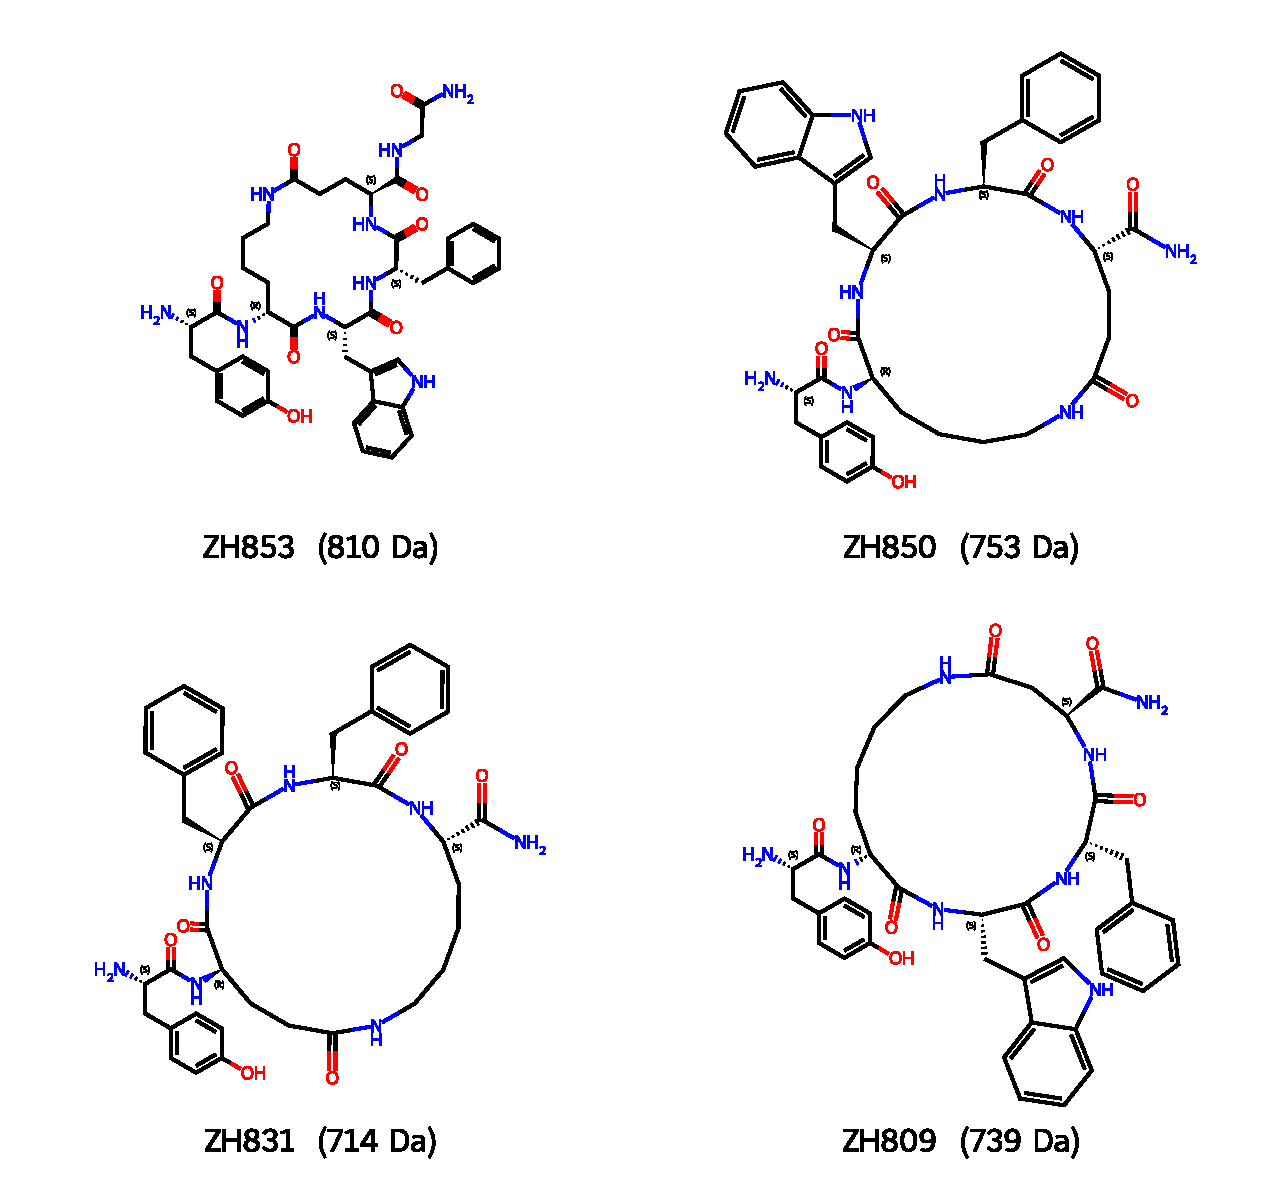
\includegraphics[width=0.92\linewidth]{figures/fig4_ligand_depictions.pdf}
  \caption{ZH853 and the three FEP analogs (ZH850/831/809), drawn as scaffold-aligned 2D structures
  with standard atom coloring and CIP stereo descriptors. All are Tyr-cyclo[\ldots]-NH$_2$ endomorphin-1
  macrocycles differing by single-residue substitutions (Trp$\leftrightarrow$Phe, Glu$\leftrightarrow$Asp
  ring size, $\pm$Gly cap).}
  \label{fig:ligands}
\end{figure}

\begin{figure}[htbp]
  \centering
  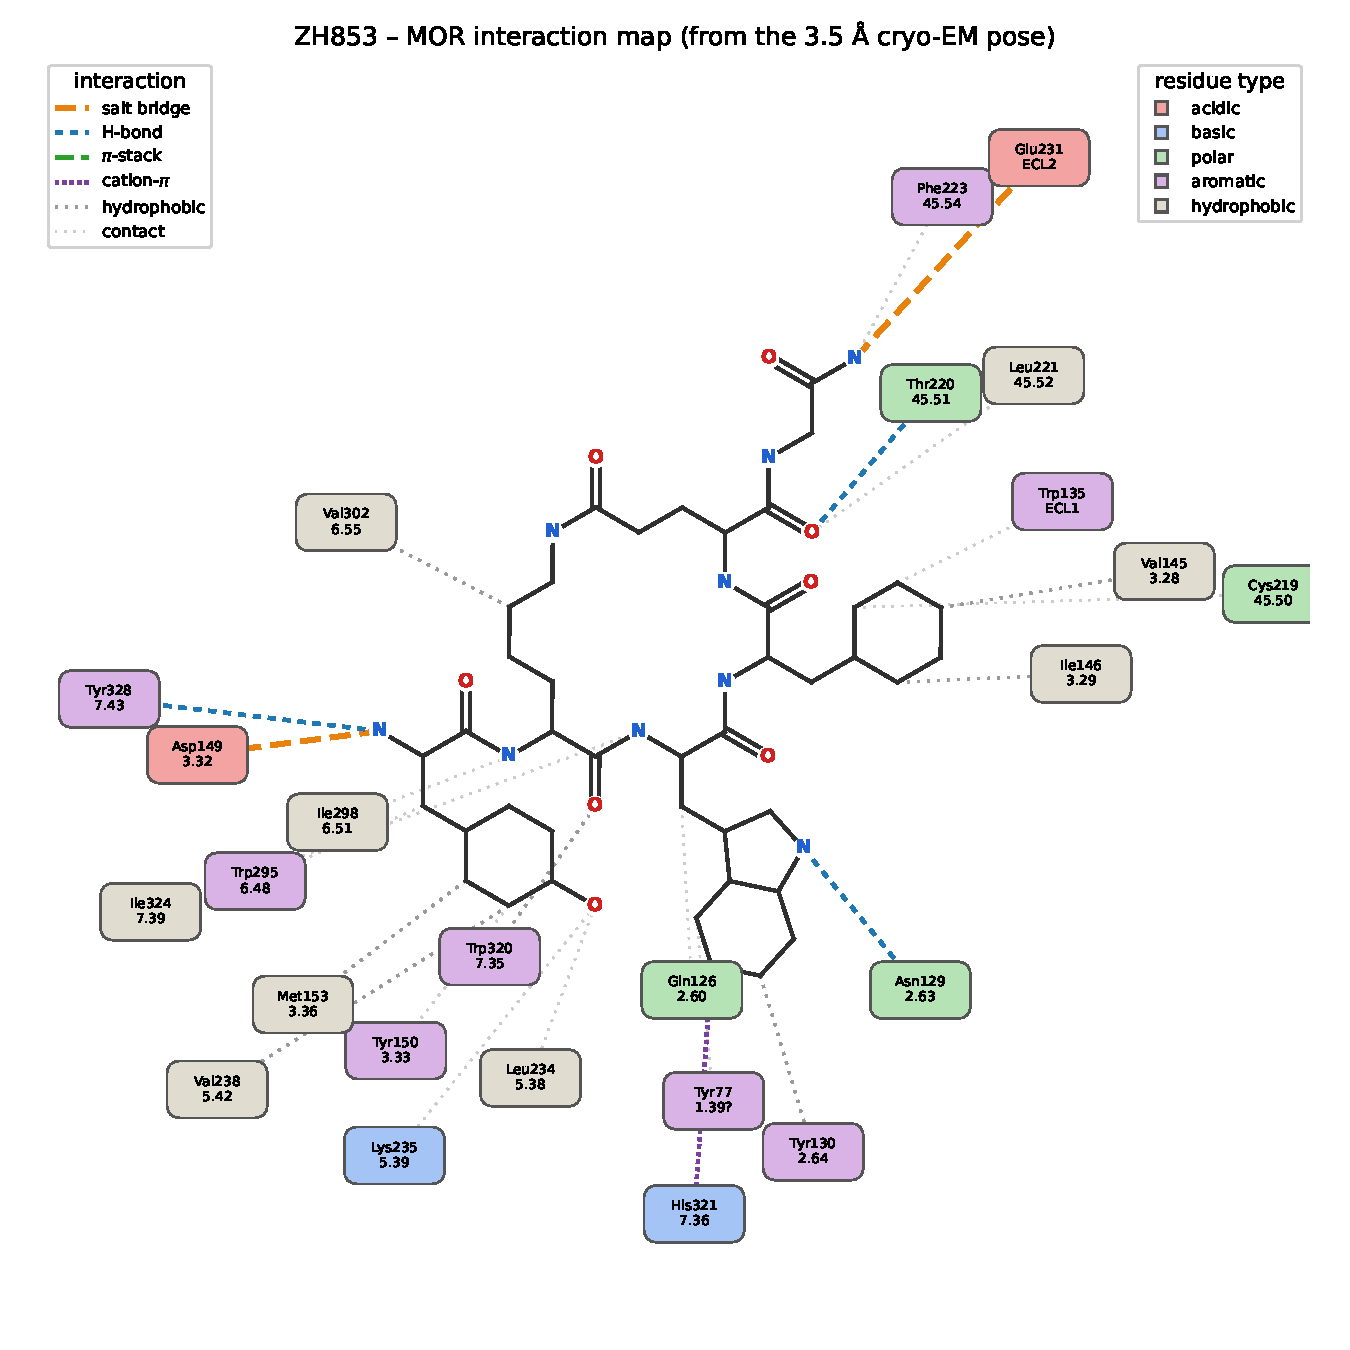
\includegraphics[width=0.92\linewidth]{figures/fig5_interaction_map.pdf}
  \caption{PoseView-style 2D interaction map of ZH853 in the MOR pocket, generated from the
  3.5\,\Ang{} cryo-EM coordinates. The ligand skeleton (atom-colored) is surrounded by contacting
  residues, colored by chemical class and placed in the direction of their contact atom; connectors
  are styled by interaction type. The Asp3.32 (Asp149) and ECL2 Glu231 salt bridges (orange) and the
  Tyr7.43/Asn2.63 H-bonds (blue) are highlighted.}
  \label{fig:posemap}
\end{figure}

\begin{figure}[htbp]
  \centering
  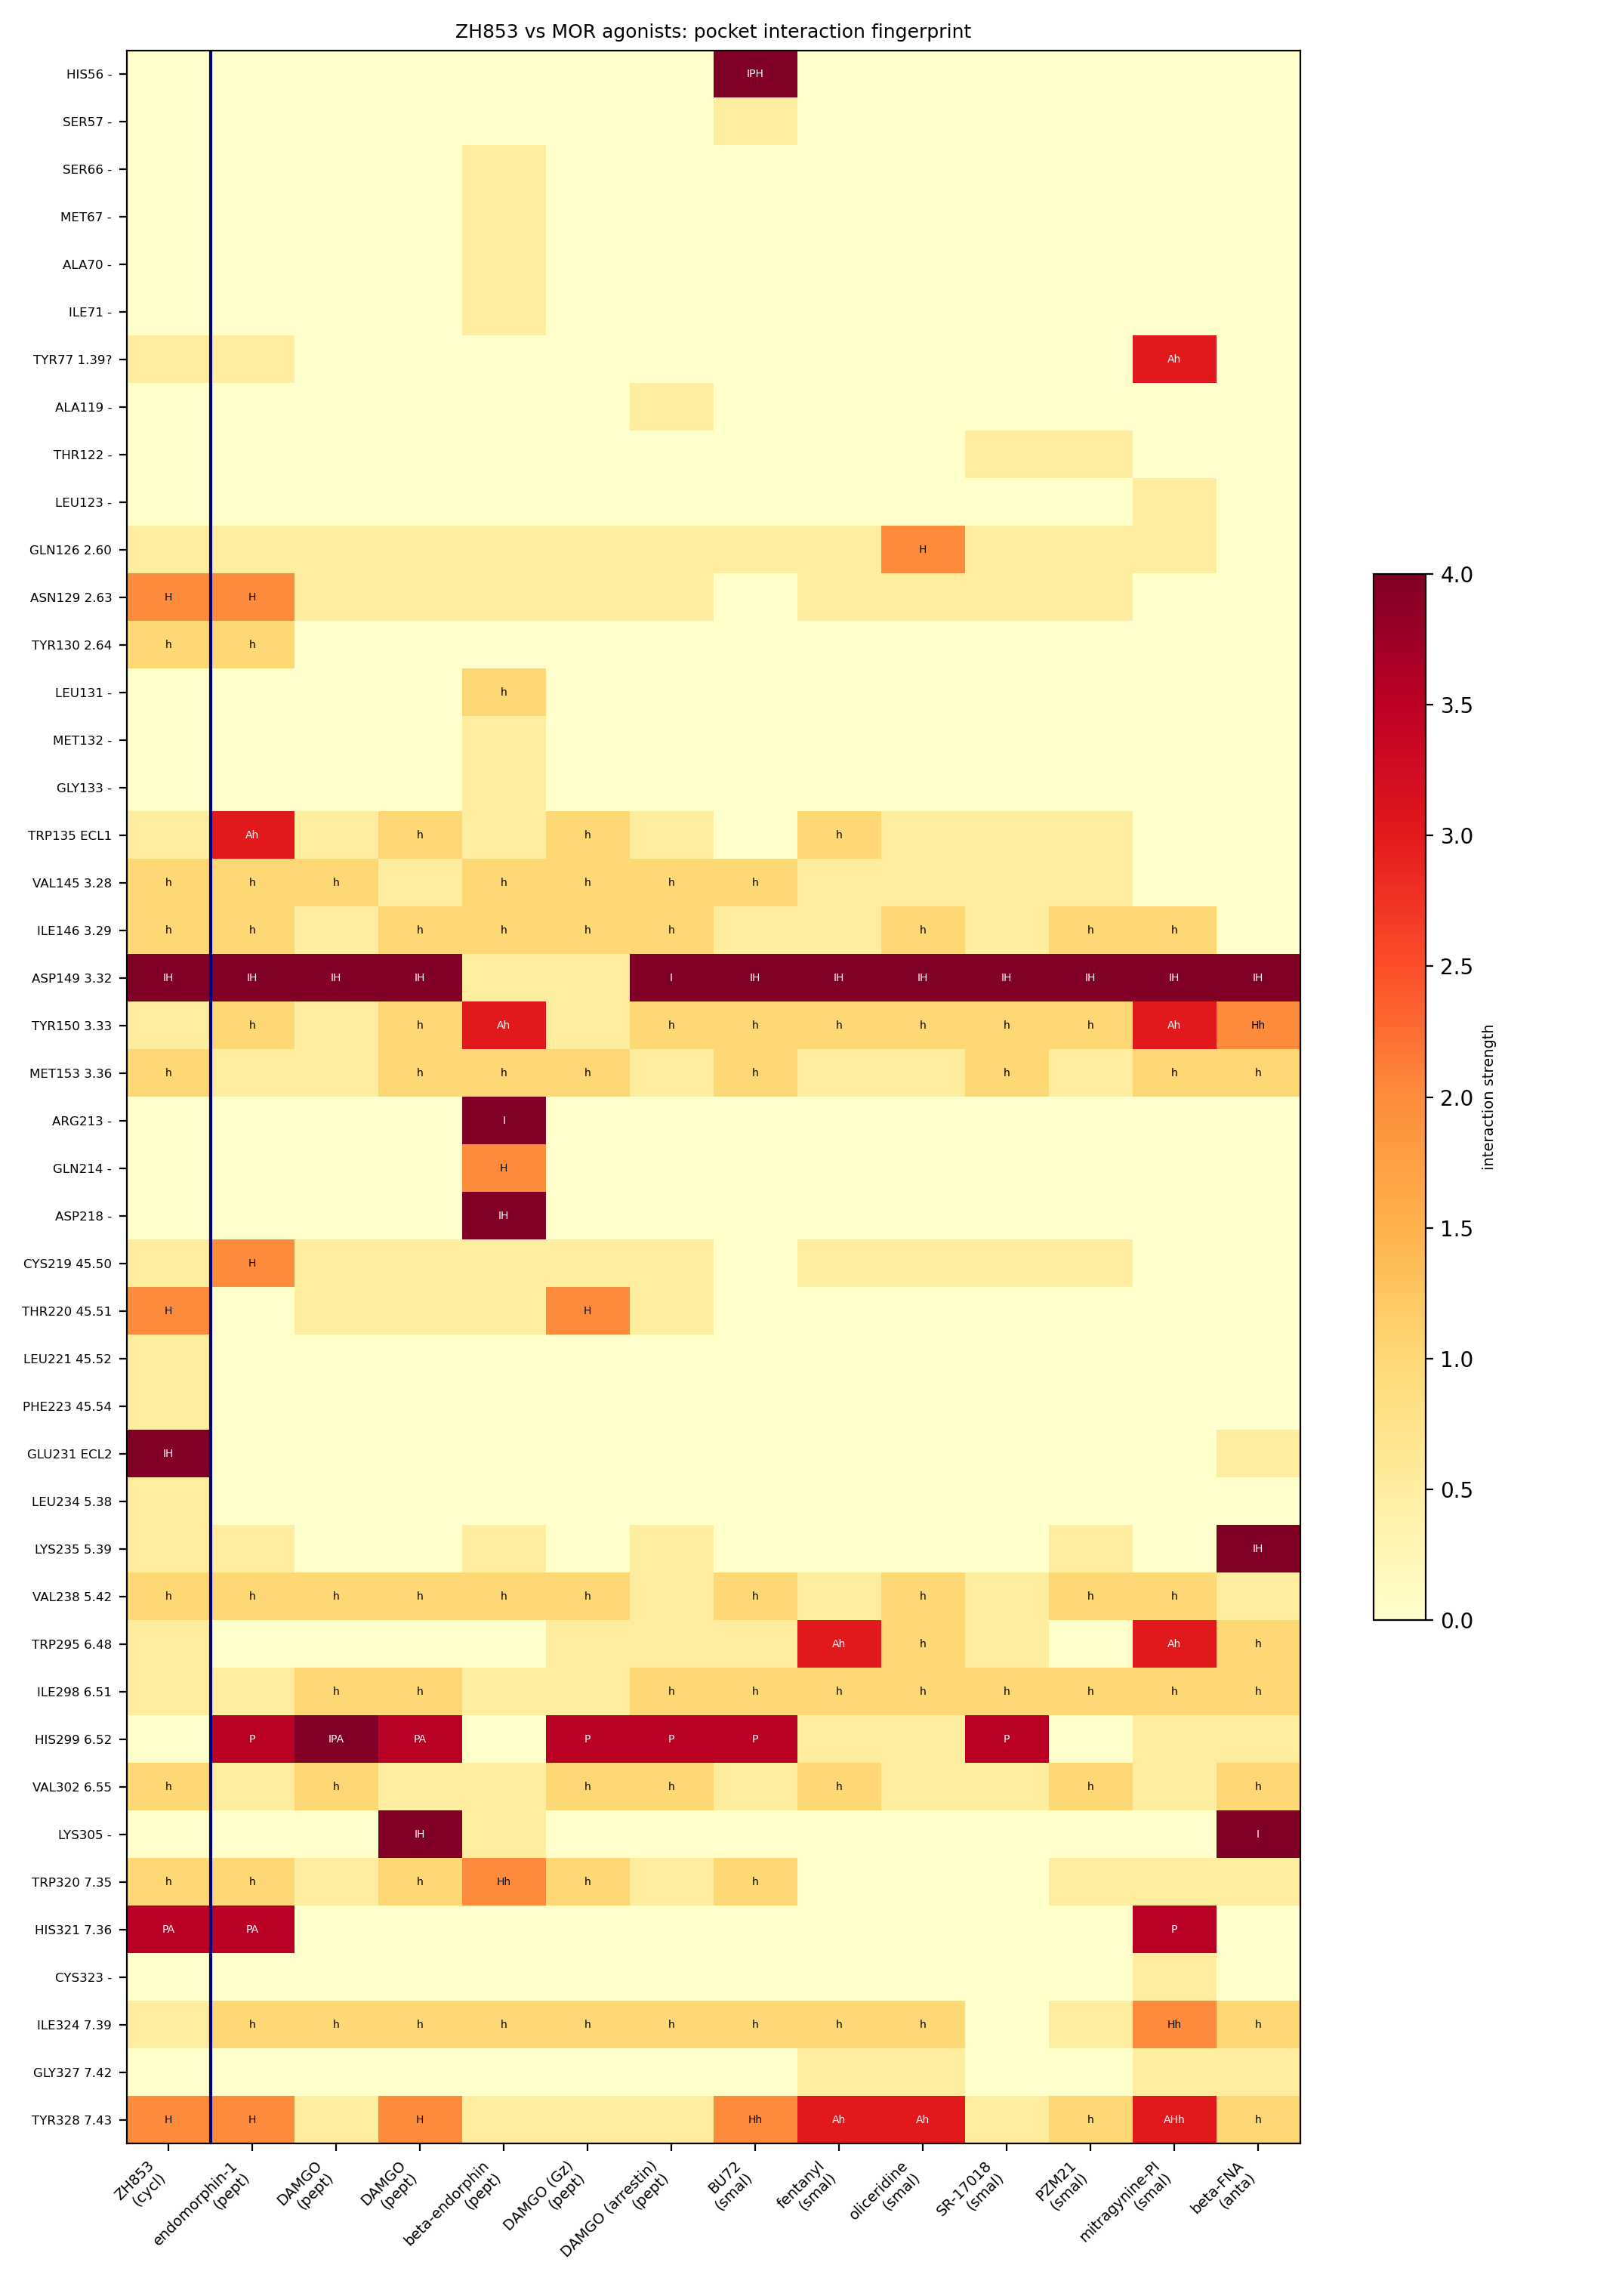
\includegraphics[width=0.85\linewidth]{figures/fig1_interaction_heatmap.png}
  \caption{Pocket interaction fingerprint of ZH853 vs 13 MOR complexes. Rows = receptor residues
  (human OPRM1 / Ballesteros-Weinstein); columns = complexes; cells colored by interaction strength
  and labeled by type (I ionic, P cation-\pistack, A \pistack-stack, H H-bond, h hydrophobic). Asp3.32
  is engaged across all columns; Glu231 (ECL2) is engaged in the ZH853 column alone.}
  \label{fig:heatmap}
\end{figure}

\begin{figure}[htbp]
  \centering
  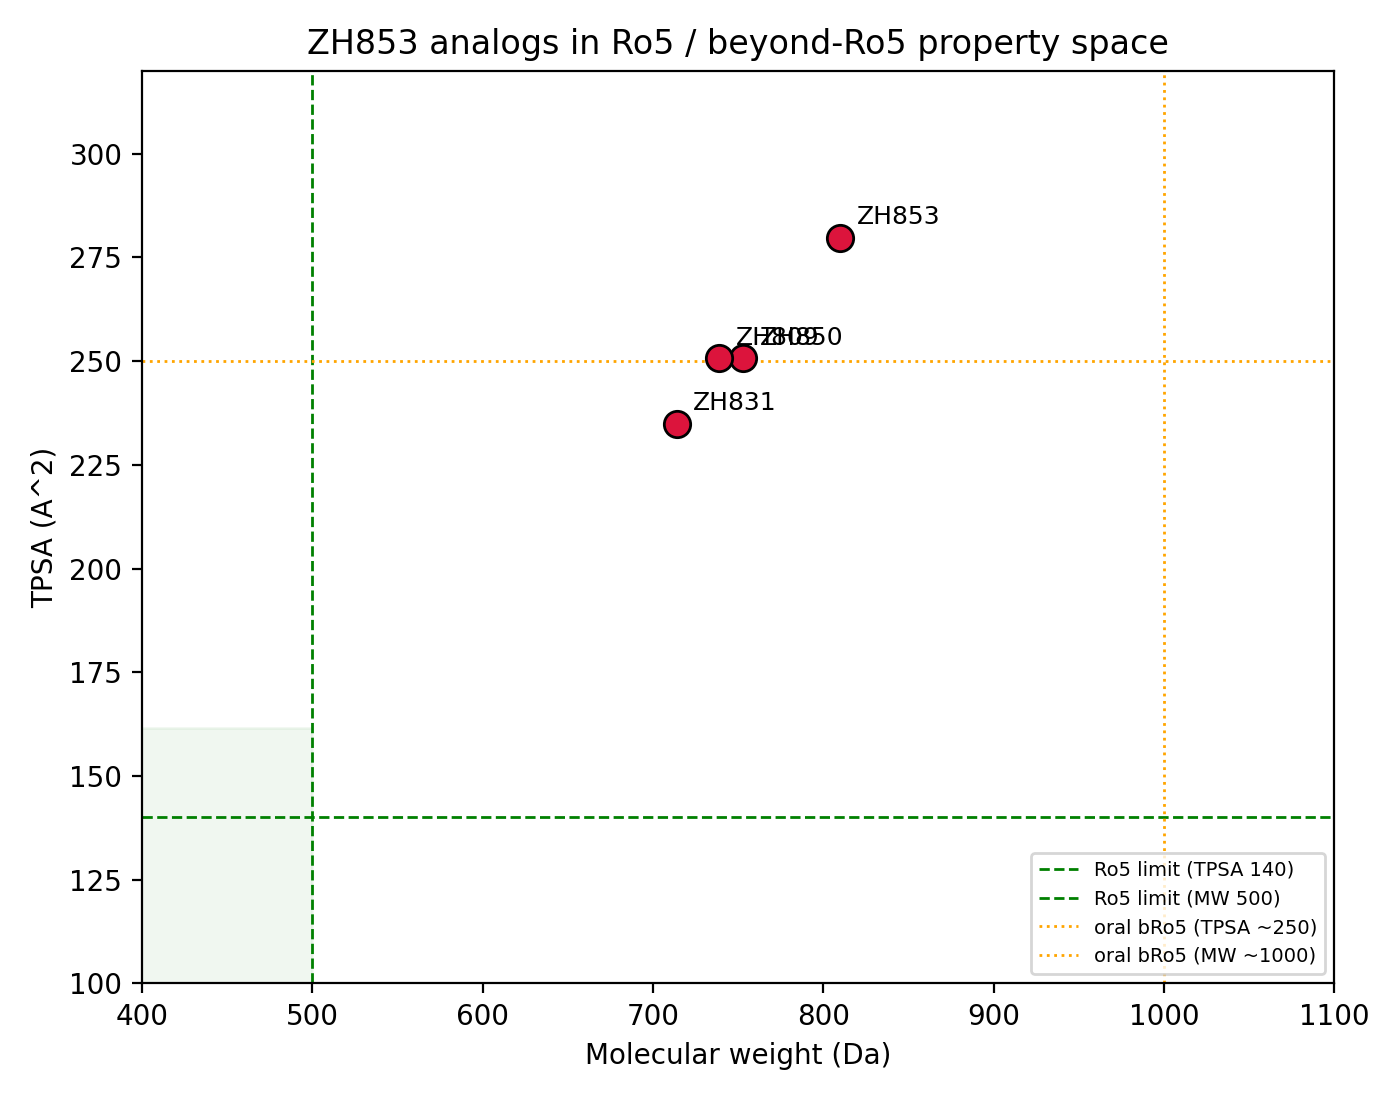
\includegraphics[width=0.7\linewidth]{figures/fig2_property_space.png}
  \caption{ZH853 analogs in Ro5 / beyond-Ro5 property space (MW vs TPSA), with Lipinski and oral-bRo5
  reference limits.}
  \label{fig:props}
\end{figure}

\begin{figure}[htbp]
  \centering
  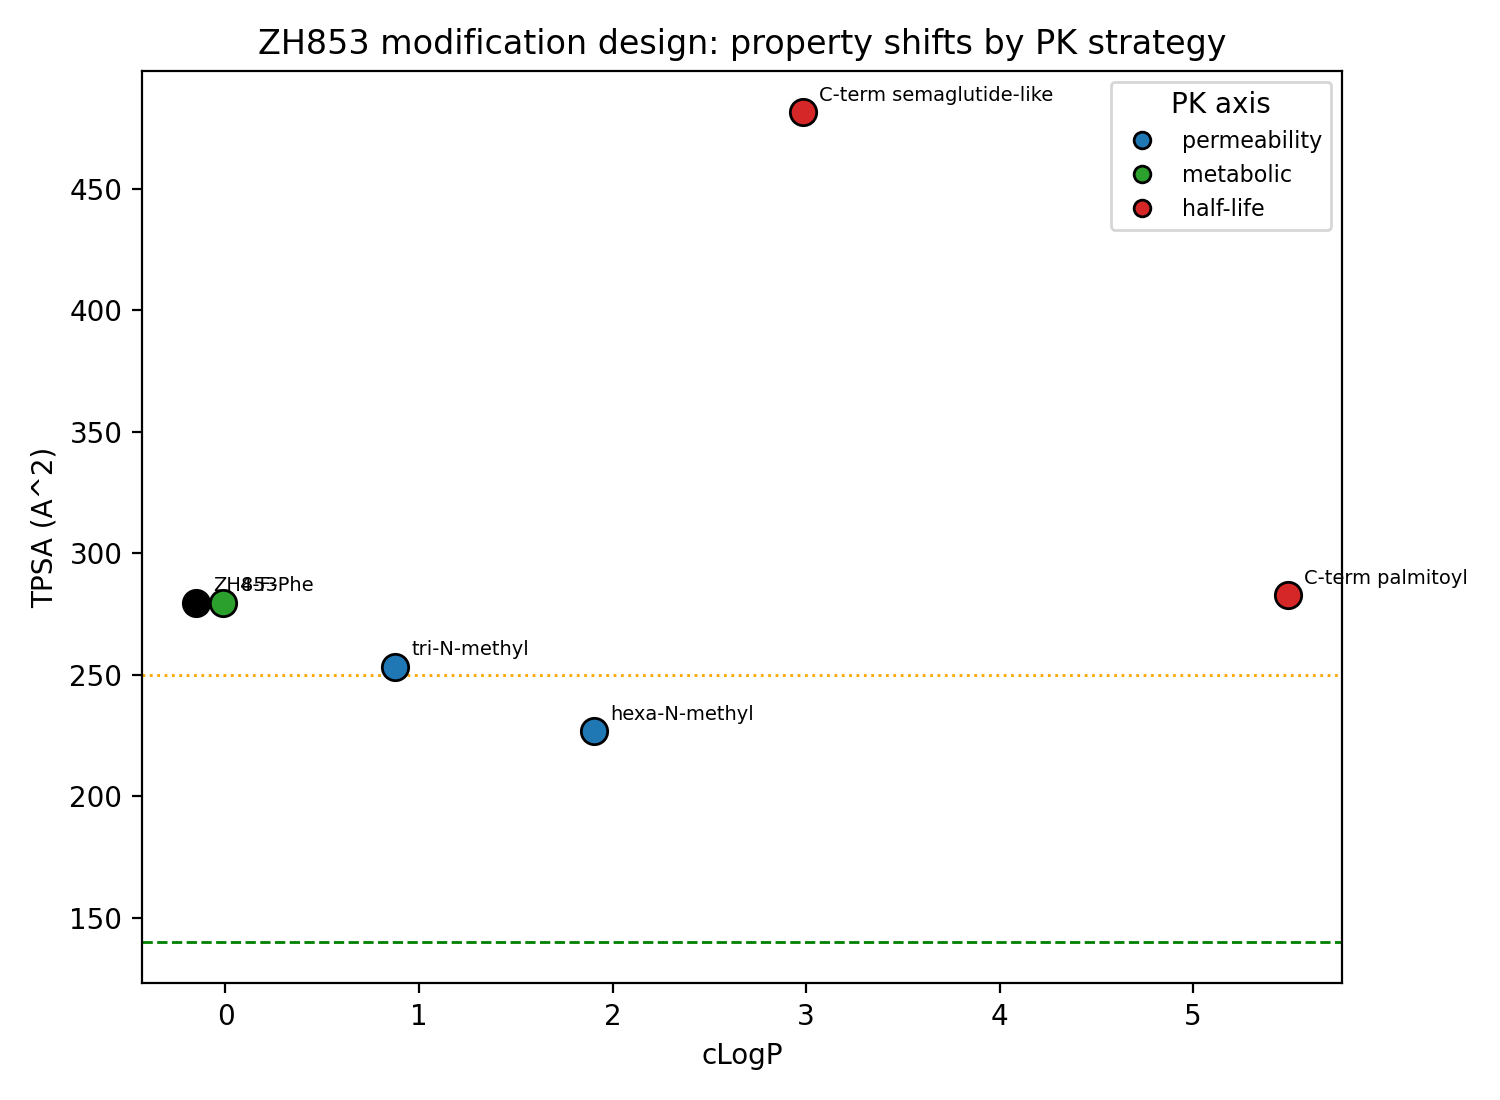
\includegraphics[width=0.75\linewidth]{figures/fig3_design_shifts.png}
  \caption{Predicted property shifts of the modification strategies by PK axis (TPSA vs cLogP):
  N-methylation (permeability) lowers TPSA across the bRo5 line; lipidation (half-life) raises
  lipophilicity.}
  \label{fig:design}
\end{figure}

\begin{table}[htbp]
  \centering
  \caption{ZH853 contacts ranked by distinctiveness (excerpt). Full interaction matrix and mutation
  panel are provided as dated \texttt{product/} outputs (Data and code availability).}
  \label{tab:distinctive}
  \footnotesize
  \setlength{\tabcolsep}{4pt}
  \begin{tabular}{@{}llp{2.9cm}cp{4.3cm}@{}}
    \toprule
    Residue & BW & ZH853 interaction & \#/12 & Note \\
    \midrule
    Glu231 & ECL2 & ionic + H-bond & \textbf{0} & ZH853-unique; primary selectivity handle
      (E231Q/E231A) \\
    His321 & 7.36 & \pistack-stack + cation-\pistack & 2 & shared only with endomorphin-1, mitragynine \\
    Tyr130 & 2.64 & hydrophobic & 1 & endomorphin-1 only \\
    Leu221/Phe223 & 45.52/45.54 & contact & 0 & weak ECL2 contacts (cyclic scaffold) \\
    Asp149 & 3.32 & ionic + H-bond & 12 & universal anchor --- do-not-mutate control \\
    Tyr328 & 7.43 & H-bond & 12 & universal (3--7 lock) --- control \\
    \bottomrule
  \end{tabular}
\end{table}

\section*{Data and code availability}

\sloppy
All analyses are scripted and version-controlled in the project repository (\texttt{src/}, numbered
workflows; \texttt{zh853mor} package; \texttt{make analysis} reproduces every figure and table).
Comparator structures are re-fetchable via \texttt{make fetch}. Decisions and clarifications are logged
in \texttt{SPECIFICATION.md}; detailed methods and results are in the \texttt{docs/} directory
(\texttt{METHODS\_md\_prep}, \texttt{RESULTS\_interactions}, \texttt{RESULTS\_analog\_design}).
\fussy

\begin{thebibliography}{99}
\small
\bibitem{zadina2016} Zadina JE, et al. Endomorphin analog analgesics with reduced abuse liability.
  \emph{Neuropharmacology} 2016. doi:10.1016/j.neuropharm.2015.12.024
\bibitem{manglik2012} Manglik A, et al. Crystal structure of the \uor{} receptor bound to a morphinan
  antagonist. \emph{Nature} 2012;485:321. (4DKL)
\bibitem{huang2015} Huang W, et al. Structural insights into \uor{} receptor activation.
  \emph{Nature} 2015;524:315. (5C1M)
\bibitem{koehl2018} Koehl A, et al. Structure of the \uor{} receptor--Gi protein complex.
  \emph{Nature} 2018;558:547. (6DDE/6DDF)
\bibitem{zhuang2022} Zhuang Y, et al. Molecular recognition of morphine and fentanyl by the \uor{}
  receptor. \emph{Cell} 2022;185:4361. (8EF5/8EF6/8EFB/8EFL/8EFO/8EFQ)
\bibitem{qu2023} Qu Q, et al. Insights into distinct signaling profiles of the \uor OR.
  \emph{Nat Chem Biol} 2023;19:423. (7T2G/7T2H)
\bibitem{wang2023} Wang Y, et al. Structures of the entire human opioid receptor family
  (endomorphin-1/\bt-endorphin). \emph{Cell} 2023;186:413. (8F7R/8F7Q)
\bibitem{zhang2025} Zhang Y, et al. Structures of MOR with Gz and \bt-arrestin. \emph{Cell Res}
  2025;35:1021. (9WST/9WSV)
\bibitem{doak2014} Doak BC, et al. Oral druggable space beyond the rule of 5. \emph{Chem Biol}
  2014;21:1115.
\bibitem{whitty2016} Whitty A, et al. Quantifying the chameleonic properties of macrocycles.
  \emph{Drug Discov Today} 2016.
\bibitem{knudsen2019} Knudsen LB, Lau J. The discovery and development of semaglutide.
  \emph{Front Endocrinol} 2019;10:155.
\end{thebibliography}

\end{document}
